\section{Data verification}
%Why checksum
Wireless communication is prone to noise and shit\cite{source}. To be able to discern correct packets from incorrect packets, a detection method is necessary. There are multiple ways to verify a packet's integrity and this section will contain a description of some methods and the reasoning behind the selected solution.

\subsection{Definition and types}
%What is a checksum
A checksum is a unique value that can be used to verify that a message is received correctly \cite{datapakke}. The checksum is based on all parts of the message and unique to the resolution of the checksum. 
A single bit checksum can only distinguish between two messages, and is not able to verify with more than 50\% accuracy, as an error could affect the transferred message so that the checksum calculation still produces the same checksum. Checksums can variate by multiple properties, for example by how it is calculated or by its length. 

\subsection*{Digit sum} \todo{Source? Example?}
A simple algorithm for producing a checksum is to use the digit sum and store it in a byte. This algorithm is efficient, but has several flaws, therein the uniqueness of the checksum of only 256 values and that two bit flips could cancel each other out and cause the same checksum. The error detection level is regarded as too small, and the this algorithm will not be used in the protocol.

\subsection*{MD5}
MD5 is a widespread checksum algorithm. It produces a 128 bit checksum, which is 16 bytes. MD5 is designed to run efficiently on 32 bit processors, which is a disadvantage on the Arduino boards used in the solution, since these posses an 8 bit processor. The 16 byte checksum uses half of the possible payload of the nRF24L01, and makes the protocol less scalable to other systems. \todo{how?} The MD5 algorithm is therefore discarded as the checksum generator for this project. \cite[p.~308]{boyles2010ccna}.

\subsection*{Cyclic redundancy check}
Another checksum algorithm is cyclic redundancy check/code, hereafter referenced to as \textit{CRC}. This exists in several forms, based on the parameters. The checksum size is variable as well as internal algorithm parameters. \todo{wat} CRC can detect single error, more than a single error and burst error \cite[p.~31]{elahi2001network}. The CRC meets the criteria for the solution, hence the selected checksum generator is CRC.

\subsection{Computation of a checksum}
%Calculation of a checksum
The algorithm for generating a CRC checksum is described in this subsection.
In short, the CRC executes a division of the message on a polynomial, and the remainder is used as the checksum. 
The CRC algorithm requires both sender and receiver to agree upon a generator polynomial in advance.

A message $M$ is viewed as a polynomial with binary coefficients, by treating each character in $M$ bit-wise. This makes for a relatively large number, but the decimal equivalent is irrelevant for the computation. M's length in bits is called $m$, which in example in \tabref{string} is 24.

\begin{table}[h!]
	\centering
	\begin{tabular}{ll}
		String  & CRC                        \\
		Binary  & 01000011 01010010 01000011 \\
		Decimal & 4,411,971                  \\
		Polynomial & $x^{22} + x^{17} + x^{16} + x^{14} + x^{12} + x^{10} + x^{6} + x^{1} + x^{0}$
	\end{tabular}
	\caption{String equivalents}
	\label{tab:string}
\end{table}

A generator polynomial of degree $r$ generates an $r$ bit checksum. The generator polynomial is the dividend which generates a quotient and a remainder for the message. Some polynomials are prone to creating multiple similar remainders, while others generate mostly unique remainders and it is therefore advantageous to use already developed, tested and implemented polynomials.

The execution of the division itself is done by binary long division of the polynomial representation of the message by the generator polynomial. This is done without carries and means that any bit $x^k$ is not affected by the bits $x^{k+1}$ or $x^{k-1}$. This kind of division propagates to be an \textit{exclusive or} function, as seen in \tabref{binaryxor}, applied from left to right on all bits within the length of the polynomial through the message and only when the leftmost bit in the message is 1. To illustrate the algorithm, an example of the division can be seen in \figref{crccalc}.

\begin{table}[h!]
	\centering
	\begin{tabular}{c|ll}
		$\pm$ & 0 & 1 \\
		\hline
		0   & 0 & 1 \\
		1   & 1 & 0
	\end{tabular}
	\caption{Binary addition and subtraction without carries.}
	\label{tab:binaryxor}
\end{table}


\begin{figure}[!h]
	\centering
	\makebox[\textwidth][c]{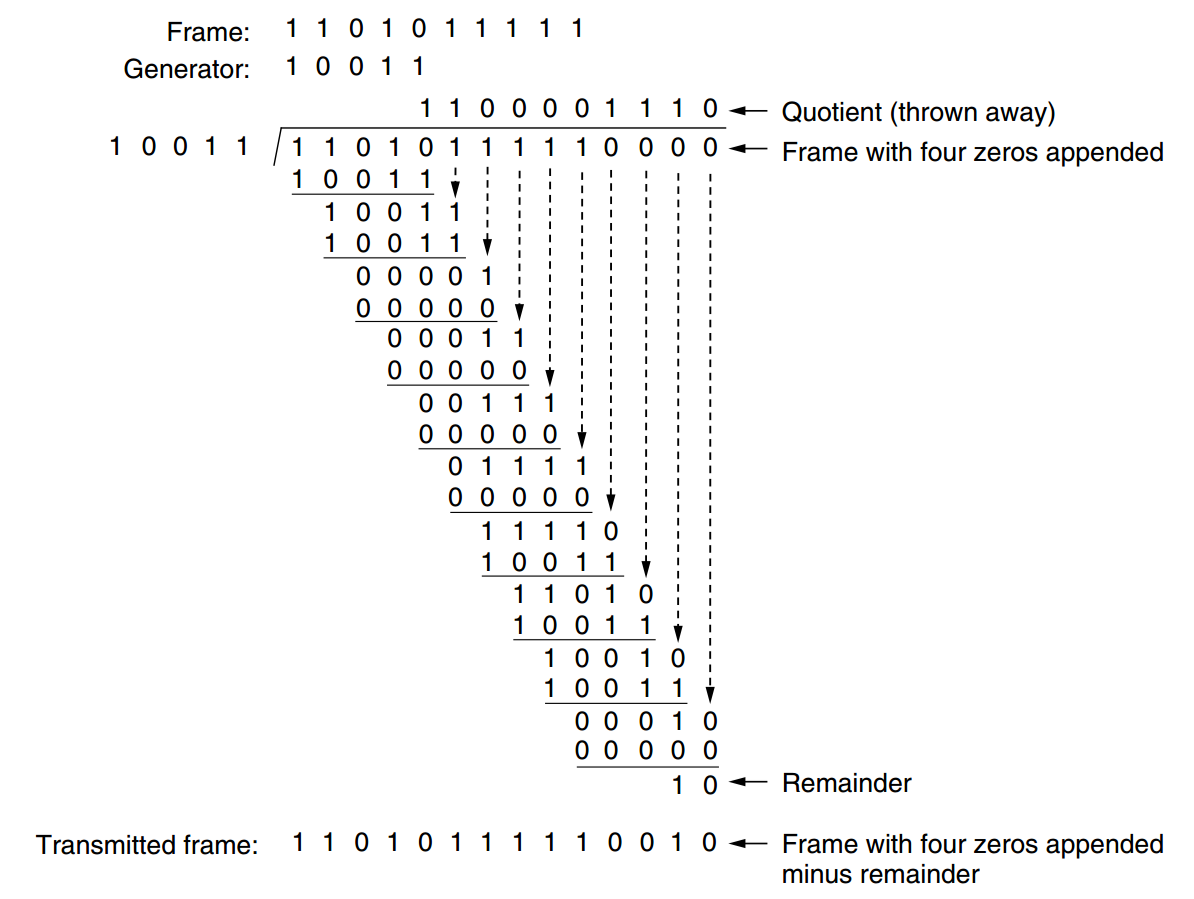
\includegraphics[width=1\textwidth]{chapters/design/figures/crc-calc.png}}	
	\caption{An example of binary long division \cite{tanenbaum81}, where ''Frame'' equals message.}
	\label{fig:crccalc}
\end{figure}

The algorithm for generating a transfer message is the following, when a message $M$, a size $r$ of the checksum and a polynomial $G$ is decided:
\begin{enumerate}
	\item For degree $r$ of $G$: append $r$ zeroes to the lower end of M, s.t. $M+R = Mx^r$
	\item Divide $Mx^r$ by $G$, using binary division
	\item Subtract remainder from $Mx^r$ using binary subtraction, resulting in transfer message $T$
\end{enumerate}

\begin{align}
	Mx^r - QG &= R \label{eq:remainder} \\
	Mx^r - R  &= QG \\
	Mx^r - R  &= T \\
	T &= QG \\
\end{align}

Result $(Mx^r - R = T)$ is the transfer message, made by the operations $(Mx^r) / G = R$ and $Mx^r - R = T$.

The equation for the checksum is shown here. $M$ minus some quotient/multiple of the generator polynomial $G$ leaves a remainder $R$, as seen in equation \ref{eq:remainder}. 

% notes
\iffalse
\begin{align}
	Mx^r - QG &= R \label{eq:remainder} \\
	Mx^r - R  &= QG \\
	Mx^r &= QG + R
\end{align}


prerequisites:
r bit CRC checksum requires degree r generator polynomial.
m bit message

M = polynomial representation of the message(binary)
R = polynomial representation of the remainder calculated by the sender
Q = quotient discarded, as only R is necessary

Sent message (transmitted data) = Mx$^r$ - R

$Mx^r = QG + R$

algorithm:
1. r degree of G: append r zeroes to the lower end of M, s.t. $M+R = Mx^r$
2. divide $Mx^r$ by G, using mod 2/binary division
3. Subtract remainder from $Mx^r$ using binary subtraction
Result $(Mx^r - R = T)$ is the transfer message

$Mx^r / G = R$
$Mx^r - R = T$
\fi
% /notes
